\section*{Instrucciones:}

La tarea se entrega y se resuelve en equipos de máximo 3 integrantes (1 a 3 personas). La tarea se entrega virtualmente en formato pdf tanto si son fotos de cuaderno, está realizada en word, en LATEX, etc.

No habrán reposiciones de tareas. Las tareas se pueden entregar con máximo 2 días de retraso para ser evaluadas sobre 8.

\textbf{Puntos Totales: 100}

\textbf{Tiempo estimado: $\approx$ 2hrs}

\section*{Ejercicios}

\begin{enumerate}
    \item Contesta de forma breve (máximo 3 líneas por pregunta) lo siguiente:

    \begin{enumerate}
        \item ¿Cuál es la diferencia entre una historia secuencial y una concurrente?

        
        
        \item Describe con tus propias palabras, ¿en qué consiste la linealizabilidad?

        
        
        \item Describe con tus propias palabras, ¿cuál es la diferencia entre la consistencia secuencial y la linealizabilidad?

        
    \end{enumerate}

    \item ¿La siguiente propiedad es equivalente a decir que un objeto x es wait-free?
    Argumenta por qué.
    
    \textbf{Propiedad:} Para toda historia infinita H de x, cada hilo que toma un número infinito de pasos en H completa un número infinito de llamadas a métodos. 

    \item Considera la siguiente ejecución de una implementación de una pila para tres hilos p, q, r y sobre un solo objeto (de tipo pila).
    
    La especificación secuencial de una pila es que el método push(x) añade a x al inicio de la pila y el método pop() : x elimina el primer elemento x al inicio de la pila (mantiene \textit{LIFO}).

    \begin{center}
        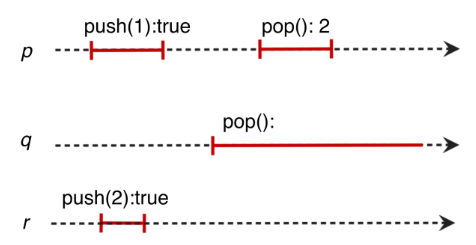
\includegraphics[width = 12 cm]{Images/Pregunta3_3.png}
    \end{center}

    \begin{enumerate}
        \item ¿Es linealizable con respecto a una pila? De ser así, incluye una 
        linearización y especifica la extensión de H y complete(H').

        \item ¿Es secuencialmente consistente? Incluye una historia que lo justifique.

        \item ¿Es consistente en la inactividad? Incluye una historia que lo justifique.
    \end{enumerate}

    \item Considera la siguiente ejecución de una implementación de una pila para dos hilos p, q y sobre dos objetos (de tipo pila) A, B. (Considera la especificación secuencial del ejercicio 2)

    \begin{center}
        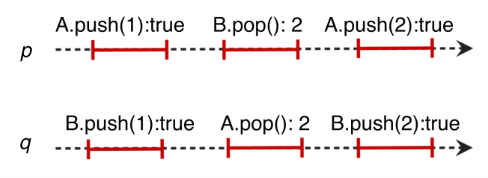
\includegraphics[width = 12 cm]{Images/Pregunta4_3.png}
    \end{center}

    \begin{enumerate}
        \item Considera que H es la historia de la ejecución, ¿H$\vert$A y H$\vert$B son secuencialmente consistentes?

        \item Considera que H es la historia de la ejecución, ¿H$\vert$A y H$\vert$B son linealizables?

        \item ¿La historia H es secuencialmente consistente y linealizable?
    \end{enumerate}

    \item Considera la siguiente clase \textit{Visibility}:

    \begin{center}
        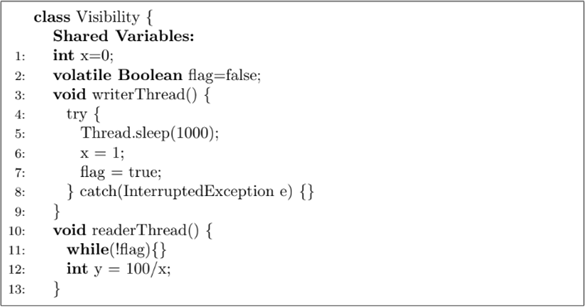
\includegraphics[width = 12 cm]{Images/Pregunta5_3.png}
    \end{center}

    \begin{enumerate}
        \item ¿Es posible que el método readerThread() divida entre cero? Argumenta porqué.

        \item Si ambas variables son volatile, ¿es posible que el método readerThread() divida entre cero?
        
        Argumenta porqué.

        \item Si ninguna de las dos variables es volatile, ¿es posible que el método readerThread() divida entre cero? Argumenta porqué.
    \end{enumerate}
    
\end{enumerate}